\chapter{Fienberg and the Evolving Role of Statistics in the Courts}
\label{ch:fienberg}

\section{A statistician in public life}

Stephen Fienberg spent most of his career at Carnegie Mellon University, where he worked on categorical data analysis, log linear models, Bayesian methods, privacy and the census. He also spent an unusual amount of time on the problems of courts and government. He analysed the December 1969 draft lottery (for 1970 induction) and showed that it had not been random \citep{fienberg1971}. He co-chaired the National Research Council's Panel on Statistical Assessments as Evidence in the Courts, whose report, \emph{The Evolving Role of Statistical Assessments as Evidence in the Courts}, appeared in 1989 under his editorship \citep{fienberg1989}. He chaired the Council's committee on the polygraph, whose 2003 report remains the most comprehensive scientific assessment of lie detection \citep{nrc2003}. With Margo Anderson he wrote \emph{Who Counts?}, a history and analysis of the political and legal fights over adjusting the United States census \citep{anderson1999}. And with Jay Kadane he wrote one of the first careful discussions of how Bayesian analyses should be presented in legal proceedings \citep{fienberg_kadane1983}.\index{Fienberg, Stephen}

This chapter is organised around Fienberg's report and the themes it established: how statistical evidence enters litigation, the problems of the adversarial expert, the use of court appointed experts, and the special difficulties of evidence about groups. We then look at four of the domains where Fienberg's own work had legal consequences: jury selection, the draft lottery and the census, and the polygraph.

\section{The 1989 report}

\subsection{Origins and method}

The panel was convened in the mid-1980s, when statistical evidence had become common in American litigation, especially in employment discrimination and antitrust, but when courts and lawyers had little guidance on how to evaluate it. The panel included statisticians, lawyers and judges. Its method was empirical: it studied a set of cases in which statistical evidence had played a large role, examining the expert reports, the testimony and the courts' opinions, and drew lessons from them. The case studies covered employment discrimination litigation, an antitrust price fixing case in which damages were estimated by regression, an environmental dispute in which the evidence concerned risks to health, and identification evidence in a criminal case.

\subsection{Findings}

The panel's main findings, stated in our own words, were these.
\begin{enumerate}[label=(\roman*)]
\item Statistical evidence was becoming more common and more complex, and courts were often ill equipped to evaluate it.
\item The adversarial system tended to produce opposing experts whose analyses differed less in method than in assumptions, and courts found it hard to decide between them.
\item Courts frequently misinterpreted significance tests, treating p values as probabilities that a hypothesis was true and statistical significance as legal significance.
\item The quality of statistical work presented in court varied widely, and professional standards for expert statisticians were weak.
\item Court appointed experts, under Rule 706 of the Federal Rules of Evidence, were underused, and could help courts understand technical disputes.
\item Bayesian methods had a natural place in legal reasoning but required care in presentation.
\end{enumerate}
Each finding remains relevant. The second deserves particular attention.\index{expert witnesses!adversarial}

\section{The adversarial expert}

In a common law trial each party selects and pays its own experts. An expert who reaches conclusions unfavourable to the party that retained her is unlikely to be called. The experts the court hears are therefore a selected sample from the population of possible expert opinions, selected by the parties for favourability. This is a statistical problem, and the panel recognised it as such.

Model it as follows. Let $\theta$ be the true answer to a technical question, such as the damages caused by a price fixing conspiracy. A competent expert, making reasonable choices of method and assumptions, reports $\theta + \epsilon$, where $\epsilon$ reflects those choices and has a distribution with mean zero and standard deviation $\sigma$. Each party consults $k$ experts and calls the one whose report is most favourable. The claimant calls the expert with the largest report, the defendant the one with the smallest. The court sees two order statistics. With normal errors, the expected gap between them grows, to leading order, like $2\sigma\sqrt{2\log k}$ for large $k$, though convergence is slow and the formula overstates the gap at small $k$. A court that splits the difference recovers $\theta$ on average, if the parties search equally hard, but cannot tell from the reports how much of the gap reflects $\sigma$ and how much the parties' search over $k$, and the reports exaggerate the real uncertainty about $\theta$.\index{selection of experts}

The panel's recommendations address this problem in several ways. Requiring experts to disclose their methods and data allows the court to see how much of the disagreement is about assumptions. Court appointed experts provide a draw from the unselected distribution. And professional standards can narrow $\sigma$ by ruling out unreasonable choices. In English procedure, the Civil Procedure Rules state that an expert's overriding duty is to the court (CPR 35.3), allow the court to direct that evidence be given by a single joint expert (CPR 35.7), and permit concurrent evidence (Practice Direction 35, paragraph 11), in which experts give evidence together and respond to each other. Each of these reforms reduces the effect of selection. A Bayesian court would go further and ask each expert to report not a point estimate but a distribution, and to state which assumptions drive it.

\section{Significance and the courts}

The panel found that courts often misread significance tests. Chapter~\ref{ch:bf} explained why: a p value is not the probability that the null hypothesis is true, and the Bayes factor implied by a p value of five per cent is modest. These errors matter most in discrimination cases, where the claim is that an employer's decisions disadvantaged a protected group, and the evidence is a comparison of the group's representation among those hired, promoted or retained with its representation among those eligible.

\subsection{Castaneda v Partida}

\begin{casebox}{Castaneda v Partida, 430 U.S. 482 (1977)}
Rodrigo Partida, a Mexican American, was convicted of burglary with intent to rape in Hidalgo County, Texas. He challenged the composition of the grand jury that indicted him, arguing that Mexican Americans had been systematically excluded. Census data showed that Mexican Americans made up about $79.1$ per cent of the county's population. Over an eleven year period, of $870$ persons summoned to serve on grand juries, only $339$, about $39$ per cent, were Mexican American. The Supreme Court held that this disparity established a prima facie case of discrimination, which the State had not rebutted \citep{castaneda1977}. In a footnote the Court explained that under random selection the expected number would be about $688$ with a standard deviation of about twelve, so the observed number was about twenty nine standard deviations below expectation, and observed that a difference of more than two or three standard deviations would make the hypothesis of random selection suspect.
\end{casebox}

The Castaneda footnote launched the two or three standard deviation rule in American discrimination law. Figure~\ref{fig:castaneda} shows the binomial distribution of Mexican American grand jurors under random selection, with the observed count far in the left tail. In this case the conclusion is not in doubt; the probability of so few Mexican Americans under random selection is astronomically small. The difficulty arises in closer cases.\index{Castaneda v Partida}

\begin{figure}[t]
\centering
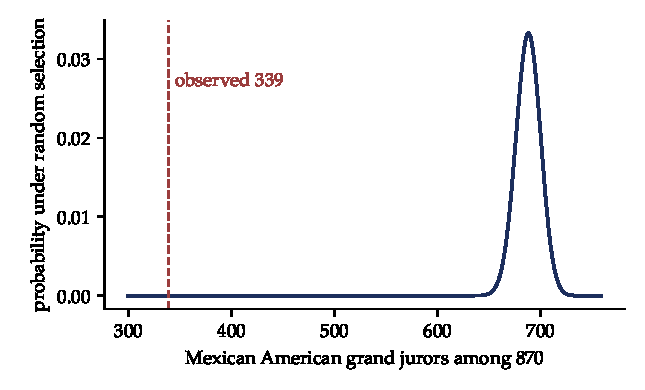
\includegraphics[width=\linewidth]{fig_castaneda}
\caption{The distribution of the number of Mexican American grand jurors among $870$ under random selection from a population that is $79.1$ per cent Mexican American, with the observed count of $339$ marked. The observed count lies about twenty nine standard deviations below the mean.}
\label{fig:castaneda}
\end{figure}

\subsection{The Bayesian analysis}

The binomial test compares the observed count with the distribution under a single hypothesis, random selection. It does not consider any alternative. A Bayesian analysis compares random selection with a hypothesis of discrimination, which must be specified. Suppose under discrimination the probability that a selected juror is Mexican American is $q$, unknown, with a prior distribution on $(0, 0.791)$. The Bayes factor for discrimination against random selection is
\begin{equation}
\BF = \frac{\int_0^{0.791} q^{339}(1-q)^{531}\,\pi(q)\,dq}{0.791^{339}\,(0.209)^{531}}.
\end{equation}
With a uniform prior on $q$, the numerator is dominated by values of $q$ near $0.39$, and the Bayes factor is of the order of $10^{141}$. Any reasonable prior gives an overwhelming result. In a closer case, say $650$ Mexican American jurors out of $870$, about $75$ per cent, which is about three standard deviations below expectation, the Bayes factor depends heavily on the prior for $q$. If discrimination is expected to produce large shortfalls, the modest shortfall is evidence against discrimination; if it is expected to produce small ones, the evidence favours it. This is Lindley's paradox in a discrimination case, and it is why the three standard deviation rule cannot be a complete test.

The Bayesian approach also addresses an issue the binomial test ignores: the relevant population. In \emph{Hazelwood School District v United States} the Court emphasised that the comparison should be with the qualified labour pool, not the general population \citep{hazelwood1977}. For grand juries, eligibility requirements such as literacy and citizenship may differ across groups. Uncertainty about the relevant base rate, as in the Dawid and Mortera analysis of uncertain match probabilities in Chapter~\ref{ch:classic}, should be represented by a prior on the base rate, and it weakens the evidence of discrimination in close cases.

\section{Jury selection and the fair cross section}

The Sixth Amendment guarantees a jury drawn from a fair cross section of the community. In \emph{Duren v Missouri} the Supreme Court set out the test: the excluded group must be distinctive, its representation in venires must be unfair and unreasonable relative to its numbers in the community, and the under representation must be due to systematic exclusion in the selection process \citep{duren1979}. Lower courts measure under representation in several ways, among them absolute disparity, the difference between the group's share in the community and in the venires, and comparative disparity, that difference divided by the group's share in the community. Each has known defects. Absolute disparity understates the problem for small groups; comparative disparity overstates it.

A Bayesian measure avoids these defects by asking a different question: how much does the observed composition of venires change the probability that the process systematically excludes the group, relative to a process that does not? Kadane, in his own work on jury challenges, analysed jury selection data in this way \citep{kadane2008}. The answer depends on the size of the samples, the plausible size of systematic effects, and the base rate, and it can be stated as a Bayes factor, which has the same meaning for large and small groups.

\section{The draft lottery}

In December 1969 the United States Selective Service held a lottery to determine the order in which men born between 1944 and 1950 would be called for military service in the Vietnam War. The 366 days of the year were written on slips, placed in capsules, and drawn from a container. Fienberg showed that the lottery was not random: men born late in the year received systematically lower, and therefore earlier, draft numbers \citep{fienberg1971}. The capsules had apparently been added to the container month by month and not adequately mixed, so December dates, added last, sat near the top. The average draft number for December birthdays was much lower than for January ones, and a simple rank correlation test rejected randomness decisively. The procedure was changed for the next lottery.\index{draft lottery}

The draft lottery is a legal case in the broadest sense. The state was allocating a heavy burden, potentially death, by a procedure whose legitimacy rested on its fairness, and fairness was defined as randomness. A Bayesian treatment would compare the hypothesis of a fair lottery with a family of alternatives in which inadequate mixing produces a trend, and would quantify the evidence for the alternative. More important than the test is the lesson: procedures that are supposed to be random, such as jury selection, case assignment to judges or the allocation of scarce public goods, must be checked, because physical randomisation is harder than it looks.

\section{The census}

The United States Constitution requires an actual enumeration of the population every ten years for the apportionment of seats in the House of Representatives. The census misses some people and double counts others, and the net undercount is larger for some groups than for others. From the 1980s onwards there were proposals to adjust the census using a post enumeration survey, a large sample survey whose results could be used to estimate and correct the undercount by dual system estimation, a capture recapture method. The proposals were fought out in Congress and in the courts.\index{census adjustment}

Anderson and Fienberg's \emph{Who Counts?} tells the story of the 1990 census and the fight over plans for 2000 \citep{anderson1999}. In \emph{Department of Commerce v United States House of Representatives} the Supreme Court held in 1999 that the Census Act prohibits the use of statistical sampling to determine the population for the purpose of apportioning representatives among the states. Sampling remained permitted for other purposes. The legal outcome turned on statutory interpretation, but the underlying dispute was about whether a statistical estimate, with known sampling error and model assumptions, was more or less accurate than an enumeration with known coverage error. A Bayesian analysis would compare the expected loss from each, with the loss defined by errors in apportionment. Fienberg's work showed how such comparisons could be made, and how political interests shaped the willingness to make them.

\section{The polygraph}

The polygraph measures physiological responses (heart rate, blood pressure, breathing and skin conductance) while a subject answers questions, on the theory that deception produces detectable arousal. It has long been excluded as evidence in most American courts, but it is widely used in security screening by government agencies. The National Research Council committee that Fienberg chaired reviewed the scientific evidence and concluded, in 2003, that polygraph testing could discriminate lying from truth telling at rates well above chance but well below perfection, in specific incident investigations with naive subjects, and that the evidence for its use in screening was much weaker \citep{nrc2003}.\index{polygraph}

The committee's most important argument was Bayesian. In employee screening, the base rate of spies among those tested is low. Even a test with high accuracy produces many more false positives than true positives when the base rate is low. Suppose a test detects ninety per cent of spies and clears ninety per cent of non spies, and one employee in a thousand is a spy. In a population of ten thousand, there are ten spies, of whom nine fail the test, and $9{,}990$ non spies, of whom $999$ fail. Of the $1{,}008$ who fail, only nine are spies, less than one per cent. Raising the threshold for failure to reduce false positives also reduces the detection rate. The committee concluded that the polygraph's accuracy in screening was insufficient to justify reliance on it for security decisions. This is the base rate argument of the cab problem in Chapter~\ref{ch:odds}, applied to national security, and it is a model of how Bayesian reasoning should inform public policy on evidence.

\section{Fienberg and Kadane on presentation}

Fienberg and Kadane's 1983 paper in \emph{The Statistician} addressed the question that Tribe had raised: how should a Bayesian analysis be presented in a legal proceeding \citep{fienberg_kadane1983}? Their answer, in brief, was that an expert should present the likelihood function, or the Bayes factor, for the evidence, and show how the posterior would vary over a range of priors, so that the fact finder can supply its own prior. They emphasised that the expert should not present a posterior probability of guilt or liability, because the prior belongs to the fact finder and because a single posterior hides the sensitivity of the conclusion. They also discussed the presentation of uncertainty about the model itself.

\section{Legacy}

Fienberg died in 2016. His work on the courts showed that statisticians could improve legal decisions not by replacing lawyers' reasoning with formulas but by making the structure of the reasoning explicit, testing whether procedures did what they claimed, and insisting on base rates. Chapter~\ref{ch:kadane} turns to his collaborator Jay Kadane, whose work as an expert witness gives a closer view of Bayesian statistics in the courtroom.

\section*{Notes and Questions}
\addcontentsline{toc}{section}{Notes and Questions}
\begin{enumerate}[label=\arabic*.]
\item Verify the Castaneda footnote: compute the mean and standard deviation of the binomial distribution with $n = 870$ and $p = 0.791$, and the number of standard deviations by which $339$ falls short.
\item Compute the Bayes factor for discrimination in a close case of $650$ out of $870$, with a uniform prior on $q$ over $(0.5, 0.791)$ and over $(0.7, 0.791)$. Discuss.
\item In the adversarial expert model, suppose each party consults five experts and calls the most favourable. With $\sigma = 1$, compute by simulation the expected gap between the reports. What would a court learn from a single joint expert?
\item In the polygraph example, find the base rate at which half of those who fail the test are spies.
\item Read \emph{Duren v Missouri}. Propose a Bayesian test for the second element and compare it with absolute and comparative disparity on a small and a large group.
\item The December 1969 draft lottery used physical randomisation. Propose a test of randomness that a court could apply to the assignment of cases to judges. What alternatives should it be powerful against?
\end{enumerate}

\section*{Further reading}
Fienberg's report \citep{fienberg1989}; Fienberg and Kadane on presentation \citep{fienberg_kadane1983}; Anderson and Fienberg on the census \citep{anderson1999}; the polygraph report \citep{nrc2003}; and Finkelstein and Levin's \emph{Statistics for Lawyers} for many worked cases \citep{finkelstein2015}.
